% explains why yours is the best possible design
% helps others avoid dead ends
%
% your final design is typically the result of exploring a tree
%
% keep intro and walkthrough short by explaining only 
% in a separate design section mention dead ends
% do not drill deeper into dead ends though
%
\section{Design}
%
To create our device we used five techniques 
to observe the target groups needs and funnel those 
into an ever more refined design. 
\begin{description}
  \item[User Study] We never intended to win new customers to 
    the social-web idea, instead we focused on customers already 
    using services like Twitter\trademark or Facebook\registered. 
    We believe that social networks are the Web 2.0 killer application. 
    Customers are flocking to them at the same time, mobile devices
    become increasingly more popular, so demand for a union of 
    those has risen considerably, as we found out during our preliminary 
    user study.
  \item[Contextual Inquiry]
    During our contextual inquiry we were able to identify some stereotypical 
    target users and created common task descriptions those users would 
    attempt most often. While the user focus seems to differ largely, ranging 
    from staying in touch using messages to just using them as an automtic 
    birthday reminder, all of them used the messaging functionality and 
    shared photos with their friends. 
\begin{figure}[h]
  \begin{center}
    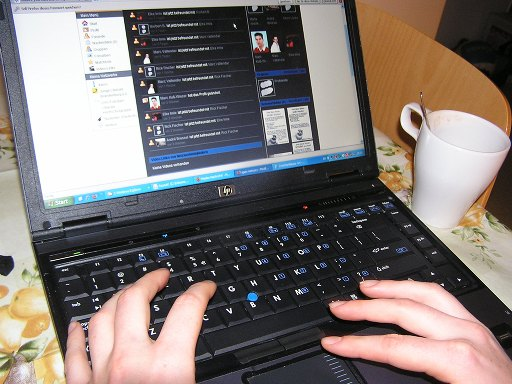
\includegraphics[width=0.8\linewidth]{imgs/context.png}
  \end{center}
  \caption{The Typical Use of a Social Network}
  \label{fig:context}
\end{figure}
  \item[Task Analysis]
    In order to further specify the tasks we want to offer with the SociaPath
    we prepared a questionnaire for our target audience. After completing the 
    survey, we had identified a final set of tasks our users perform most often. 
    Additionally, we asked the users what the users perceive
  \item[Functionality and Design]
\begin{figure}[h]
  \begin{center}
    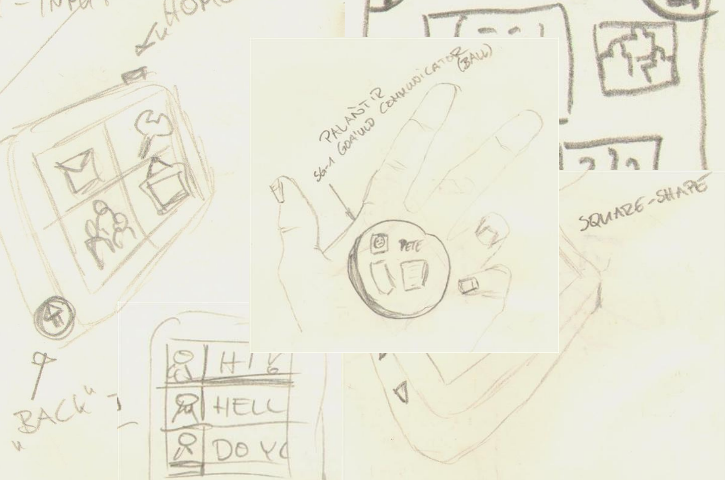
\includegraphics[width=0.8\linewidth]{imgs/sketches.png}
  \end{center}
  \caption{A Selection of Sketches for Interface Studies}
  \label{fig:sketches}
\end{figure}
  \item[Usability Flaws and Paper Prototyping]
    Used a link map.
  \item[Interactive Prototype]
\begin{figure}[h]
  \begin{center}
    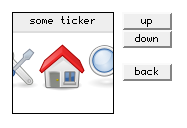
\includegraphics[width=0.8\linewidth]{imgs/screen.png}
  \end{center}
  \caption{A Screenshot of the Interactive Prototype}
  \label{fig:prototype}
\end{figure}
\end{description}
